% Fig 3.18 Ce3+ (4f1) level diagram: free ion (L=3, S=1/2) -> spin-orbit
% (J=7/2 / J=5/2, ~0.3 eV) -> axial crystal-field Kramers doublets
% (physically ordered: |+/-1/2> top ... |+/-7/2> bottom, fixing the duplicated
% printed labels) -> Zeeman split of the ground |+/-5/2> doublet, 0.1 meV.
\documentclass[tikz,border=5pt]{standalone}
\usetikzlibrary{arrows.meta}
\usepackage{amsmath}
\usepackage{bm}
\usepackage{fontspec}
\setmainfont{Times New Roman}
\begin{document}
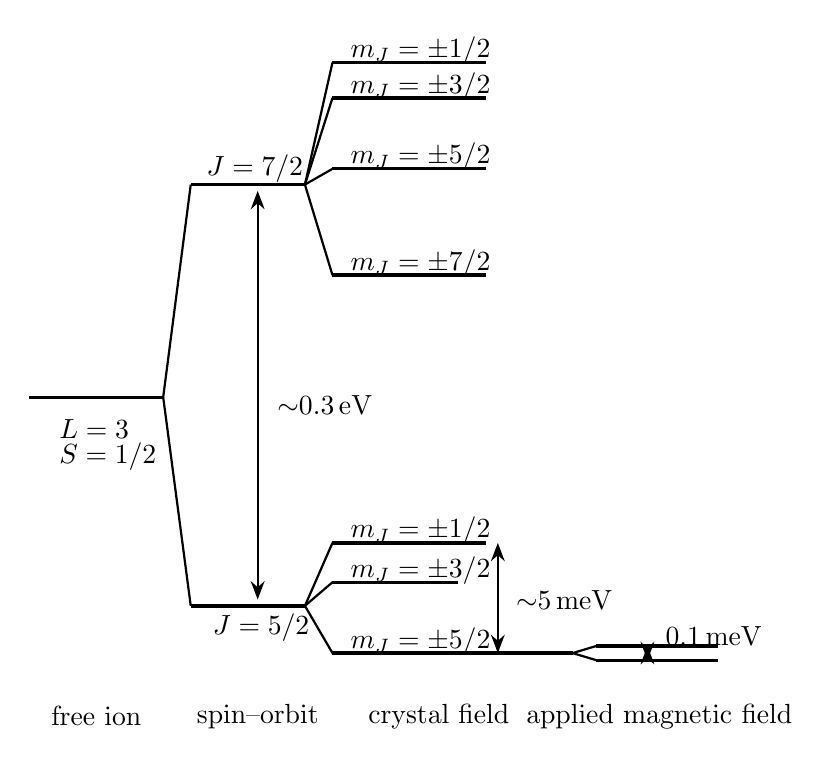
\begin{tikzpicture}[line width=0.8pt,>=Stealth]
% ---------- free ion ----------
\draw[very thick] (0.1,4.2) -- (1.8,4.2);
\node[anchor=west] at (0.35,3.80) {$L=3$};
\node[anchor=west] at (0.35,3.45) {$S=1/2$};
% fan to spin-orbit levels
\draw (1.8,4.2) -- (2.15,6.9);
\draw (1.8,4.2) -- (2.15,1.55);
\draw[very thick] (2.15,6.9) -- (3.6,6.9);
\node[anchor=west] at (2.22,7.10) {$J=7/2$};
\draw[very thick] (2.15,1.55) -- (3.6,1.55);
\node[anchor=west] at (2.3,1.28) {$J=5/2$};
% ~0.3 eV double arrow
\draw[<->] (3.0,6.82) -- (3.0,1.63);
\node[anchor=west] at (3.12,4.1) {$\sim$0.3\,eV};
% ---------- crystal field: J=7/2 -> four doublets ----------
\draw (3.6,6.9) -- (3.95,8.45);
\draw (3.6,6.9) -- (3.95,8.00);
\draw (3.6,6.9) -- (3.95,7.10);
\draw (3.6,6.9) -- (3.95,5.75);
\draw[very thick] (3.95,8.45) -- (5.9,8.45);
\draw[very thick] (3.95,8.00) -- (5.9,8.00);
\draw[very thick] (3.95,7.10) -- (5.9,7.10);
\draw[very thick] (3.95,5.75) -- (5.9,5.75);
\node[anchor=west] at (4.05,8.60) {$m_J=\pm 1/2$};
\node[anchor=west] at (4.05,8.15) {$m_J=\pm 3/2$};
\node[anchor=west] at (4.05,7.25) {$m_J=\pm 5/2$};
\node[anchor=west] at (4.05,5.90) {$m_J=\pm 7/2$};
% ---------- crystal field: J=5/2 -> three doublets ----------
\draw (3.6,1.55) -- (3.95,2.35);
\draw (3.6,1.55) -- (3.95,1.85);
\draw (3.6,1.55) -- (3.95,0.95);
\draw[very thick] (3.95,2.35) -- (5.90,2.35);
\draw[very thick] (3.95,1.85) -- (5.55,1.85);
\draw[very thick] (3.95,0.95) -- (7.00,0.95);
\node[anchor=west] at (4.05,2.50) {$m_J=\pm 1/2$};
\node[anchor=west] at (4.05,2.00) {$m_J=\pm 3/2$};
\node[anchor=west] at (4.05,1.10) {$m_J=\pm 5/2$};
% ~5 meV crystal-field scale on the J=5/2 manifold
\draw[<->] (6.05,2.35) -- (6.05,0.95);
\node[anchor=west] at (6.15,1.62) {$\sim$5\,meV};
% ---------- applied field: ground doublet split ----------
\draw (7.00,0.95) -- (7.30,1.04);
\draw (7.00,0.95) -- (7.30,0.86);
\draw[very thick] (7.30,1.04) -- (8.85,1.04);
\draw[very thick] (7.30,0.86) -- (8.85,0.86);
\draw[<->] (7.95,1.04) -- (7.95,0.86);
\node[anchor=west] at (8.05,1.17) {0.1\,meV};
% ---------- stage names ----------
\node at (0.95,0.15) {free ion};
\node at (3.00,0.15) {spin--orbit};
\node at (5.30,0.15) {crystal field};
\node at (8.10,0.15) {applied magnetic field};
\end{tikzpicture}
\end{document}
